\documentclass{article}

\usepackage[ngerman]{babel}
\usepackage[utf8]{inputenc}
\usepackage[T1]{fontenc}
\usepackage{hyperref}
\usepackage{csquotes}
\usepackage[a4paper]{geometry}
\usepackage{graphicx}

\usepackage[
    backend=biber,
    style=apa,
    sortlocale=de_DE,
    natbib=true,
    url=false,
    doi=false,
    sortcites=true,
    sorting=nyt,
    isbn=false,
    hyperref=true,
    backref=false,
    giveninits=false,
    eprint=false]{biblatex}
\addbibresource{../references/bibliography.bib}


\title{Ist es ethisch vertretbar, KI für die Erstellung von Kunst zu verwenden?}
\author{Noah Cooper}
\date{\today}


\begin{document}

\maketitle

\abstract{
    In dieser Arbeit beschäftige ich mich damit, wie künstliche Intelligenz in der Welt der Kunst verwendet wird und gehe der Frage nach, ob dies ethisch vertretbar ist.
}

\tableofcontents

\newpage

\section{Einleitung}
\label{sec:introduction}

Ist es ethisch vertretbar, KI für die Erstellung von Kunst zu verwenden? Mit dieser Leitfrage beschäftige ich mich in der folgenden Arbeit. 
Künstliche Intelligenz hat die Welt im Sturm erobert. Völlig logisch, denn sie arbeitet noch personalisierter und effizienter als eine einfache Suchmaschine, was in unserer heutigen Gesellschaft sehr gefragt ist. Auch im Bereich der Kunst sieht es nicht anders aus. Aber wem gehören die Urheberechte, wenn hinter einer Kreation gar kein Mensch steckt? Und welche Auswirkungen kann das auf unser aktuelles Verständnis der Kunst haben?

\section{Wie wird KI trainiert?}
    Laut yukosai.com kann das Training einer KI in mehrere Schritte unterteilt werden:
    \begin{enumerate}
        \item Vorbereitung der Trainingsdaten: Auswahl einer großen Anzahl von Bildern als Basis für das Training.
        \item Labeling der Daten: Jedes Bild wird mit entsprechenden Labels versehen, um dem Modell mitzuteilen, welcher Stil oder welches Genre repräsentiert wird.
        \item Aufbau des neuronalen Netzwerks: Das Modell wird so konfiguriert, dass es die gewünschten künstlerischen Merkmale erlernen kann.
        \item Training des Modells: Durch mehrere Iterationen werden die Gewichte im Netzwerk angepasst, um die Genauigkeit und Qualität der generierten Kunstwerke zu verbessern.
        \item Auswertung und Anpassung: Nach dem Training wird das Modell auf seine Leistung überprüft und gegebenenfalls weiter optimiert.
    \end{enumerate}
    Die KI, vor allem ausserhalb des Bereiches Kunst, bildet sich immer weiter, indem sie selbstständig Informationen aufnimmt und diese nutzt. Aus den Daten, mit denen sie gefüttert wird, kann sie neue Inhalte erstellen. Ihre Antworten basieren dabei kurz gesagt auf Wahrscheinlichkeiten, die die KI aus dem eigenen Datenmaterial ermittelt. \Citep{zdf} 
    \newline Sie kann nicht selber kreativ denken, sondern arbeitet primär mit der Erkennung und Wiederverwendung von Mustern (pattern recognition). Die Medienkunst- und Digitalexpertin Sabine Himmelsbach sagt in einem Interview mit SRF: "Künstliche Intelligenz besitzt weder poetische noch intuitive Ansätze, die für Kunstschaffende von zentraler Bedeutung sind. Sie operiert lediglich nach deren Handlungsanweisungen." \Citep{srf}
    
    \subsection{Wie gut ist die KI-Kunst?}  
    Mit einem AI Image Generator lässt sich jedes Bild erstellen, das man sich nur wünschen könnte. 
        An Qualität lassen sie aber oft zu wünschen übrig. 
        KI-Kunst kann auch ziemlich verstörend sein, wie das Beispielbild weiter unten zeigt: Auf den ersten Blick sieht es aus wie ein mystisches oder märchenhaftes Bild von einer Elfe, die von merkwürdigen Gestalten verfolgt wird. Diese Idee wird einem auch sehr gut vom Bild vermittelt. Sobald man aber genauer hinsieht, merkt man, dass die Proportionen überhaupt nicht passen: Des Mädchens Finger wachsen an komischen Stellen aus ihren Händen; ihre Ohren sehen total komisch aus und ihr Hals ist kaum vorhanden. Die Gestalten hinter ihr haben zum Beispiel drei Augen oder man erkennt gar nicht, wo ihre Nasen sind. 
        \begin{figure}[ht]
        \centering        
        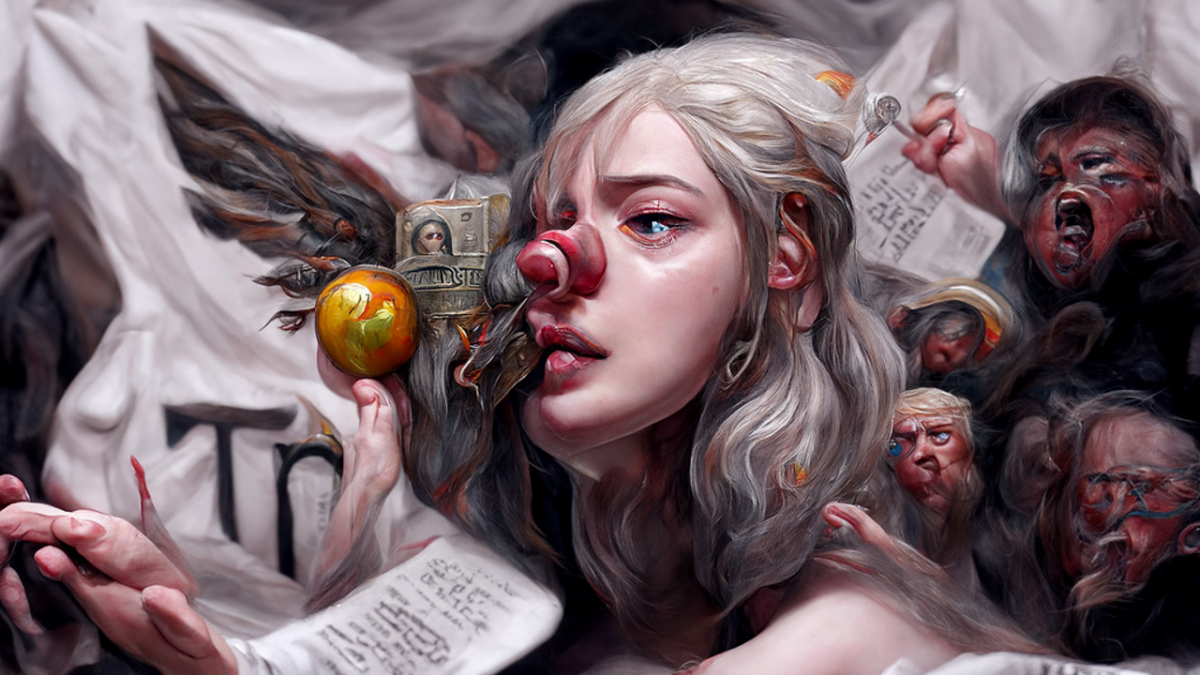
\includegraphics[width=0.8\textwidth]{ki-bild.png} 
        \caption{A detailed painting of an allegory of truth and lies - Disco Diffusion (Versuch 55)}
        \label{fig:ki-bild}
        \end{figure}
        Dieses Beispiel zeigt, dass die heutige gewöhnliche KI eindeutig nicht dazu in der Lage ist, realistische Kunst zu erstellen.
        \newline Die KI ist ausserdem gar nicht so lernfähig, wie man vielleicht denken würde. Laut golem.de befindet sie sich ungefähr auf diesem Stand: "Während ein Kind nach dem Ansehen und Lernen des Inhaltes Katze sehr schnell jede Katze in jeder möglichen Position – zum Beispiel mit gedrehtem Kopf – identifizieren kann, würde das Netzwerk gnadenlos scheitern, wenn die Trainingsdaten keine Bilder von Katzen in Profilansicht enthielten." \Citep{ki-golem}

\newpage
\section{Was sagen Befürworter*innen der KI-Kunst?}
    Die künstliche Intelligenz kann helfen, Kunst und Kultur zugänglicher zu machen und die kreativen 
    Prozesse von Kunstschaffenden zu unterstützen und zu beschleunigen. \Citep{unesco} Sie passt sich auch komplett an die Bedarfe und Wünsche ihrer Nutzer*innen an: KI kann jeden Auftrag entgegennehmen und bearbeiten. Dadurch sind viele Leute der Meinung, die KI erleichtere ihren Alltag und helfe ihnen, schnell zu Antworten zu kommen.
    \newline Verschiedene Unternehmen und Agenturen können auch Geld einsparen, wenn sie für Werbeplakate und Logos keine Künstler*innen beauftragen müssen, sondern einfach die KI für sich arbeiten lassen können. Ausserdem können mehr Leute an der Welt der Kunst teilnehmen, weil KI unabhängig von den eigenen künstlerischen Fähigkeiten nutzbar ist. Sie bietet auch Raum für Experimentation und Selbstfindung, weil man mit ihr neue Stile und Techniken ausprobieren kann, für die man ansonsten keine Ressourcen hätte oder die gar nicht verwirklichbar wären.
    
\section{Risiken und Fragen über Urheberechte}
    Da die KI nicht selber denken, sondern nur mit bereits prozessierten Daten arbeiten kann, verwendet sie viele urheberechtlich geschützte Dokumente. Auf Social Media gibt es hunderte von Accounts, die KI-generierte Bilder posten und dafür viel Aufmerksamkeit und Bewunderung bekommen (z.B. @troplanduniverse). Das lässt bei Einigen aber einen bitteren Nachgeschmack, weil sie finden, dass es so viele Künstler*innen gibt, die viel Energie, Geld, Zeit und Leidenschaft in ihre Kunst stecken, nur um dann in der Masse unterzugehen. Das sagt auch die kalifornische Künstlerin Karla Ortiz: "Meine Werke sind meine Identität, und zu sehen, wie das verwendet wird, um etwas zu generieren, das sich wie du anfühlt – das ist furchtbar". \Citep{deutschlandfunkkultur}
    \newline Die Kunst der KI ist auch objektiv betrachtet nicht sehr wertvoll, weil sie in unlimitierten mengen vorhanden ist. Oft steigt der Preis eines Kunstwerks an, nachdem dessen Erschaffer*in gestorben ist, weil genau diese Kunst nie wieder erstellt werden kann. Bei KI ist das nicht der Fall: Sie hat kein Zerfallsdatum und wird auch Kunstwerke, die sie zuletzt vor mehreren Jahren erschaffen hat, immer wieder herstellen können.
    \newline In den meisten Fällen wird die KI nicht als Urheberin eines Kunstwerks anerkannt, weil Urheberechte normalerweise nur von Personen oder Unternehmen besessen werden können. Sie gehören dann entweder dem/der Benutzer*in oder dem/der Entwickler*in der KI-Software.

\section{Fazit und meine eigene Meinung}
    Die Nutzung von KI ermöglicht die Erstellung faszinierender Kunstwerke, wie etwa durch KI-Bildgeneratoren. Dennoch verstehe ich die Besorgnis vieler Künstler*innen, dass ihre Arbeitsplätze und Einnahmequellen bedroht sein könnten. KI-Kunst hat ohne menschliche Überlegungen in meinen Augen weniger Wert, da sie keine selber ausgedachten Botschaften vermittelt, die kontrovers diskutiert werden können. 
    \newline Die ethische Vertretbarkeit der Nutzung von KI für die Erstellung von Kunst hängt von einer Vielzahl von Faktoren ab, darunter technologische Innovation, künstlerische Freiheit, soziale und finanzielle Auswirkungen sowie rechtliche und ethische Überlegungen. Während KI neue kreative Möglichkeiten bietet und die Kunstwelt bereichern kann, müssen Bedenken hinsichtlich der Arbeitsplatzsicherheit, der Authentizität und der kulturellen Bedeutung von Kunst ernst genommen werden. Eine ethisch vertretbare Nutzung von KI in der Kunst erfordert Transparenz, faire Praktiken und einen respektvollen Umgang mit der menschlichen Kreativität.

\printbibliography

\end{document}
